% =====================================================================
%  quizgen — Presentation slides  (FAU Erlangen corporate-design Beamer)
%  Automated Test Assembly: selecting exams from a question bank
%
%  Compile with:  pdflatex slides.tex   (run twice for the page totals)
%
%  NOTE ON BRANDING
%  ----------------
%  This deck reproduces the FAU Erlangen-Nürnberg corporate look
%  (FAU blue + FAU cyan, title/footer bands, university wordmark) in a
%  fully self-contained way, so it builds without the official FAU theme
%  package or logo files.  The two corporate colours are defined just
%  below; if you have the exact FAU corporate-design hex values (or the
%  official "FAU.svg"/"FAU.pdf" logo), drop them in there and into the
%  \fauLogo command and nothing else needs to change.
% =====================================================================
\documentclass[11pt,aspectratio=169]{beamer}

\usepackage[utf8]{inputenc}
\usepackage[T1]{fontenc}
\usepackage{lmodern}
\usepackage{amsmath,amssymb}
\usepackage{booktabs}
\usepackage{array}
\usepackage{xcolor}
\usepackage{listings}
\usepackage{tikz}
\usetikzlibrary{arrows.meta,positioning,fit,backgrounds,calc,shapes.geometric}

% ---- FAU corporate-design colours -----------------------------------
% Replace with the exact corporate hex values if you have them.
\definecolor{faublue}{RGB}{0,47,94}      % FAU primary "Hausblau"
\definecolor{faucyan}{RGB}{0,177,235}    % FAU light-blue accent
\definecolor{faugrey}{RGB}{128,128,128}
\definecolor{faulightgrey}{RGB}{236,239,241}

% diagram palette (kept consistent with the written report)
\definecolor{cstage}{RGB}{222,235,247}
\definecolor{cstageb}{RGB}{49,130,189}
\definecolor{cdata}{RGB}{229,245,224}
\definecolor{cdatab}{RGB}{49,163,84}
\definecolor{cctrl}{RGB}{253,224,221}
\definecolor{cctrlb}{RGB}{222,45,38}
\definecolor{cgrey}{RGB}{99,99,99}
\definecolor{ckw}{RGB}{0,90,160}
\definecolor{cstr}{RGB}{160,60,0}
\definecolor{ccmt}{RGB}{100,120,100}

% =====================================================================
%  Self-contained FAU-style Beamer theme
% =====================================================================
\useinnertheme{rectangles}
\setbeamertemplate{navigation symbols}{}
\setbeamertemplate{itemize items}[circle]

% palette
\setbeamercolor{structure}{fg=faublue}
\setbeamercolor{frametitle}{fg=white,bg=faublue}
\setbeamercolor{title}{fg=faublue}
\setbeamercolor{author}{fg=faublue}
\setbeamercolor{normal text}{fg=black}
\setbeamercolor{itemize item}{fg=faucyan}
\setbeamercolor{itemize subitem}{fg=faucyan}
\setbeamercolor{block title}{fg=white,bg=faublue}
\setbeamercolor{block body}{bg=faulightgrey}
\setbeamercolor{alerted text}{fg=faucyan}

\setbeamerfont{frametitle}{series=\bfseries}
\setbeamerfont{title}{series=\bfseries,size=\LARGE}
\setbeamerfont{block title}{series=\bfseries}

% FAU wordmark used top-right of every frame (swap for the real logo).
\newcommand{\fauLogo}{%
  \textbf{\textcolor{faublue}{FAU}}%
}

% --- frame title: blue band with a cyan rule underneath --------------
\setbeamertemplate{frametitle}{%
  \nointerlineskip%
  \begin{beamercolorbox}[wd=\paperwidth,ht=2.6ex,dp=1.2ex,leftskip=0.6em,rightskip=0.6em]{frametitle}%
    \insertframetitle\hfill\raisebox{-0.2ex}{\small\textcolor{faucyan}{\textbf{FAU}}}%
  \end{beamercolorbox}%
  {\color{faucyan}\rule{\paperwidth}{1.1pt}}%
}

% --- footer: thin band, author | short title | university | page ------
\setbeamertemplate{footline}{%
  \vbox{%
    \hbox{\color{faucyan}\rule{\paperwidth}{0.6pt}}%
    \hbox{%
      \begin{beamercolorbox}[wd=.30\paperwidth,ht=2.4ex,dp=1ex,leftskip=0.6em]{author in head/foot}%
        \usebeamerfont{author in head/foot}\tiny\textcolor{faublue}{J.~Hayashi}%
      \end{beamercolorbox}%
      \begin{beamercolorbox}[wd=.45\paperwidth,ht=2.4ex,dp=1ex,center]{title in head/foot}%
        \usebeamerfont{title in head/foot}\tiny\textcolor{faugrey}{quizgen — Automated Test Assembly}%
      \end{beamercolorbox}%
      \begin{beamercolorbox}[wd=.25\paperwidth,ht=2.4ex,dp=1ex,rightskip=0.6em]{date in head/foot}%
        \usebeamerfont{date in head/foot}\hfill\tiny\textcolor{faublue}{FAU Erlangen-Nürnberg \quad\insertframenumber/\inserttotalframenumber}%
      \end{beamercolorbox}%
    }%
  }%
}

% ---- listings (python / yaml / bash) --------------------------------
\lstdefinestyle{slide}{
  basicstyle=\ttfamily\scriptsize,
  keywordstyle=\color{ckw}\bfseries,
  stringstyle=\color{cstr},
  commentstyle=\color{ccmt}\itshape,
  showstringspaces=false,
  breaklines=true,
  frame=single,
  rulecolor=\color{faugrey!40},
  framesep=4pt,
  columns=fullflexible,
  keepspaces=true,
  aboveskip=4pt,belowskip=2pt,
}
\lstset{style=slide}

\newcommand{\code}[1]{\texttt{\small #1}}
\newcommand{\pkg}[1]{\texttt{\small #1}}

% ---- TikZ node styles (shared with the report) ----------------------
\tikzset{
  stage/.style={rectangle, rounded corners=3pt, draw=cstageb, fill=cstage,
                line width=0.8pt, align=center, inner sep=5pt, font=\scriptsize\bfseries,
                minimum height=9mm, minimum width=22mm},
  data/.style={rectangle, draw=cdatab, fill=cdata, line width=0.7pt,
               align=center, inner sep=4pt, font=\scriptsize, minimum height=8mm},
  ctrl/.style={rectangle, rounded corners=2pt, draw=cctrlb, fill=cctrl,
               line width=0.7pt, align=center, inner sep=4pt, font=\scriptsize},
  arr/.style={-{Stealth[length=2.2mm]}, line width=0.8pt, draw=cgrey},
}

% =====================================================================
\title{quizgen}
\subtitle{Automated Test Assembly from a Question Bank}
\author{Jiniku Hayashi}
\institute{KWARC Group \\ Friedrich-Alexander-Universität Erlangen-Nürnberg}
\date{\today}

\begin{document}

% =====================================================================
%  Title slide
% =====================================================================
{%
\setbeamertemplate{footline}{}%
\begin{frame}[plain]
  \begin{tikzpicture}[remember picture,overlay]
    % top blue band
    \fill[faublue] (current page.north west) rectangle ([yshift=-1.9cm]current page.north east);
    \node[anchor=west,text=white,font=\small] at ([xshift=0.8cm,yshift=-0.95cm]current page.north west)
      {Friedrich-Alexander-Universität Erlangen-Nürnberg \,$\cdot$\, KWARC};
    \node[anchor=east,text=white,font=\Large\bfseries] at ([xshift=-0.8cm,yshift=-0.95cm]current page.north east) {FAU};
    % cyan rule
    \fill[faucyan] ([yshift=-1.9cm]current page.north west) rectangle ([yshift=-2.0cm]current page.north east);
    % bottom cyan accent
    \fill[faucyan] (current page.south west) rectangle ([yshift=0.18cm]current page.south east);
  \end{tikzpicture}

  \vspace{2.9cm}
  \begin{flushleft}\hspace{0.4cm}%
  \begin{minipage}{0.92\textwidth}
    {\Huge\bfseries\color{faublue}quizgen}\\[2mm]
    {\LARGE\color{black}Automated Test Assembly from a Question Bank}\\[2mm]
    {\large\color{faugrey}Selecting blueprint-compliant exams from a pool of tagged questions via optimisation}\\[8mm]
    {\large\bfseries Master's Thesis — Implementation Overview}\\[5mm]
    {\normalsize\textbf{Jiniku Hayashi}\quad\textcolor{faugrey}{·}\quad Advisor: Prof.\ Michael Kohlhase}\\[1mm]
    {\small\color{faugrey}KWARC Group · FAU Erlangen-Nürnberg · \today}
  \end{minipage}
  \end{flushleft}
\end{frame}
}

% =====================================================================
\begin{frame}{Outline}
  \begin{columns}[T]
    \begin{column}{0.5\textwidth}
      \begin{enumerate}
        \item What the tool does (and does \emph{not}) do
        \item Core idea: pool, blueprint, versions
        \item The selection pipeline
        \item Data model \& the blueprint
        \item Resolving proportions to exact counts
      \end{enumerate}
    \end{column}
    \begin{column}{0.5\textwidth}
      \begin{enumerate}
        \setcounter{enumi}{5}
        \item How questions are picked (greedy / MIP)
        \item Deduplication \& validation
        \item Command-line interface
        \item Provenance of techniques
        \item Summary
      \end{enumerate}
    \end{column}
  \end{columns}
\end{frame}

% =====================================================================
\begin{frame}{What quizgen does — in one sentence}
  \begin{block}{The task}
    Given an existing \textbf{question bank} (a JSON list of tagged questions),
    \emph{select} the subset(s) that form a professor's exam, exactly matching a
    \textbf{blueprint}.
  \end{block}

  \vspace{2mm}
  \textbf{Deliberately narrow scope:}
  \begin{itemize}
    \item No question \emph{generation}. \quad No document \emph{ingestion}.
    \item Reasons only over question \emph{metadata} and the requested \emph{constraints}.
    \item \alert{No LLM, no internet} — runs fully offline.
  \end{itemize}

  \vspace{2mm}
  \begin{block}{Why this is the right framing}
    Selection becomes a \textbf{well-posed combinatorial optimisation problem}
    with an \textbf{exact, auditable} solution — unlike prompting a model to
    ``write the exam'', which couples creation with constraint satisfaction and
    gives neither guarantees nor traceability.
  \end{block}
\end{frame}

% =====================================================================
\begin{frame}{Three concepts used throughout}
  \begin{columns}[T]
    \begin{column}{0.33\textwidth}
      \begin{block}{Pool}
        Your question bank — the input JSON. Each item carries
        \textbf{chapter, difficulty, type, Bloom level}.
      \end{block}
    \end{column}
    \begin{column}{0.33\textwidth}
      \begin{block}{Blueprint}
        The exam specification: \textbf{how many}, \textbf{per chapter},
        \textbf{difficulty mix}, \textbf{allowed types}, \textbf{\#versions}.
      \end{block}
    \end{column}
    \begin{column}{0.33\textwidth}
      \begin{block}{Version}
        One assembled exam paper. Several at once — \textbf{provably sharing no
        question}.
      \end{block}
    \end{column}
  \end{columns}

  \vspace{4mm}
  \begin{center}\small
  \emph{Example:} 180-question pool $\Rightarrow$ a 20-question exam,
  10/6/4 across three chapters, an 8/8/4 easy/medium/hard mix,
  in \textbf{two disjoint versions}.
  \end{center}
\end{frame}

% =====================================================================
\begin{frame}{The selection pipeline}
  \begin{center}
  \resizebox{0.96\textwidth}{!}{%
  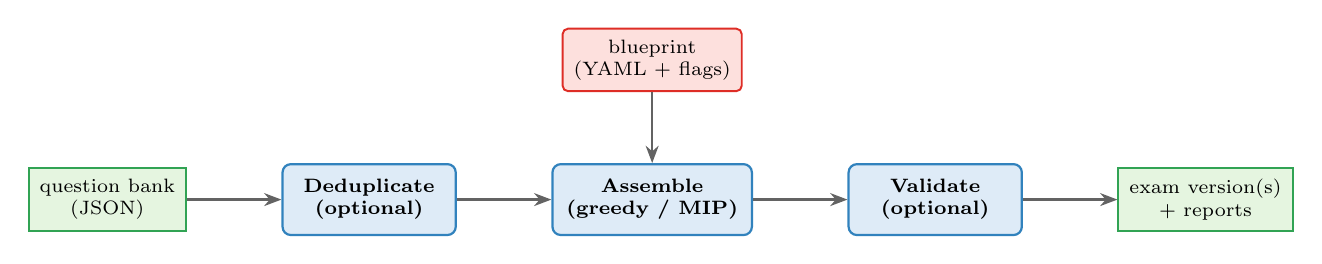
\begin{tikzpicture}[node distance=8mm and 12mm]
    \node[data] (pool) {question bank\\(JSON)};
    \node[stage, right=of pool] (dedup) {Deduplicate\\(optional)};
    \node[stage, right=of dedup] (assemble) {Assemble\\(greedy / MIP)};
    \node[stage, right=of assemble] (validate) {Validate\\(optional)};
    \node[data, right=of validate] (out) {exam version(s)\\+ reports};
    \node[ctrl, above=9mm of assemble] (bp) {blueprint\\(YAML + flags)};
    \draw[arr] (pool) -- (dedup);
    \draw[arr] (dedup) -- (assemble);
    \draw[arr] (assemble) -- (validate);
    \draw[arr] (validate) -- (out);
    \draw[arr] (bp) -- (assemble);
  \end{tikzpicture}}
  \end{center}

  \vspace{2mm}
  \begin{center}\footnotesize
  \textcolor{cdatab}{$\blacksquare$} data \quad
  \textcolor{cstageb}{$\blacksquare$} processing stage \quad
  \textcolor{cctrlb}{$\blacksquare$} professor input
  \end{center}

  \footnotesize The blueprint \textbf{drives} assembly; dedup and validation are
  opt-in. Each stage maps to one module (\pkg{schema}, \pkg{blueprint},
  \pkg{dedup}/\pkg{similarity}, \pkg{assemble}, \pkg{validate}).
\end{frame}

% =====================================================================
\begin{frame}[fragile]{Data model: the \texttt{Question} contract}
  Every artifact is a \textbf{Pydantic v2} model; the JSON Schema is
  \emph{exported} from it (so the two cannot drift).
\begin{lstlisting}[language=Python]
class Question(BaseModel):
    id: str                 # uuid4 hex[:12]
    chapter: int            # >= 1
    qtype: QuestionType     # mcq | true_false | short_answer | cloze
    bloom_level: BloomLevel # remember .. create (revised Bloom, 2001)
    difficulty: Difficulty  # easy | medium | hard
    stem: str; options: list[str] | None; answer: str
    explanation: str        # >= 10 chars
    source_ref: str         # provenance (free-form)
\end{lstlisting}
  \vspace{-1mm}
  \begin{center}\footnotesize
  \begin{tabular}{@{}ll@{}}
    \toprule
    \textbf{Field} & \textbf{Drives} \\
    \midrule
    \code{chapter} & per-chapter quotas \\
    \code{difficulty} & the easy/medium/hard mix \\
    \code{qtype} & allowed-type filtering \\
    \code{bloom\_level} & the quality objective \\
    \code{stem/answer/options} & near-duplicate detection \\
    \bottomrule
  \end{tabular}
  \end{center}
\end{frame}

% =====================================================================
\begin{frame}[fragile]{The blueprint — a ``table of specifications''}
  A small, professor-facing YAML file that translates pedagogical intent into
  measurable selection constraints:
\begin{lstlisting}
title: "AI-1 Midterm Exam"
total_questions: 20
chapters: { 1: "50%", 2: "30%", 3: "20%" }
difficulty_mix: { easy: 0.4, medium: 0.4, hard: 0.2 }
allowed_qtypes: [mcq, true_false, short_answer, cloze]
versions: 2
selector: mip            # greedy | mip
dedup_similarity: 0.85
\end{lstlisting}
  \begin{itemize}
    \item Amounts may be \textbf{exact counts} (\code{10}), \textbf{fractions}
          (\code{0.4}), or \textbf{percentages} (\code{"50\%"}).
    \item \code{versions: 2} $\Rightarrow$ two papers that \textbf{share no question}.
  \end{itemize}
\end{frame}

% =====================================================================
\begin{frame}{Resolving proportions into exact counts}
  An exam cannot contain half a question, so \code{Blueprint.resolve()} turns
  every proportional request into an integer quota \emph{before} assembly.

  \vspace{2mm}
  \begin{columns}[T]
    \begin{column}{0.5\textwidth}
      \centering\footnotesize
      \begin{tabular}{@{}lrr@{}}
        \toprule
        \textbf{Chapter} & \textbf{Share} & \textbf{Count} \\
        \midrule
        Ch.~1 & 50\% & $0.50\cdot20=10$ \\
        Ch.~2 & 30\% & $0.30\cdot20=6$ \\
        Ch.~3 & 20\% & $0.20\cdot20=4$ \\
        \midrule
        Total & 100\% & 20 \\
        \bottomrule
      \end{tabular}
    \end{column}
    \begin{column}{0.5\textwidth}
      \centering\footnotesize
      \begin{tabular}{@{}lrr@{}}
        \toprule
        \textbf{Difficulty} & \textbf{Share} & \textbf{Count} \\
        \midrule
        Easy   & 0.4 & $0.4\cdot20=8$ \\
        Medium & 0.4 & $0.4\cdot20=8$ \\
        Hard   & 0.2 & $0.2\cdot20=4$ \\
        \midrule
        Total & 1.0 & 20 \\
        \bottomrule
      \end{tabular}
    \end{column}
  \end{columns}
\end{frame}

% =====================================================================
\begin{frame}[fragile]{Largest-remainder (Hamilton) rounding}
  When shares don't divide evenly: give each category its whole part, then hand
  the leftover units to the \textbf{largest fractional remainders}.
  \[
    \text{raw}_k = w_k N,\qquad
    \text{floor}_k = \lfloor \text{raw}_k \rfloor,\qquad
    r = N - \textstyle\sum_k \text{floor}_k
  \]
  \begin{block}{Worked example: $N=21$, shares 50/30/20\,\%}
    raw $=10.5,\;6.3,\;4.2$ \;$\to$\; floors $=10,6,4$ (one left) \;$\to$\;
    largest remainder $0.5$ is Ch.~1 \;$\to$\; \textbf{11, 6, 4} (sums to 21).
  \end{block}
\begin{lstlisting}[language=Python]
def largest_remainder(weights, total):
    raw = {k: weights[k] * total for k in weights}
    counts = {k: int(raw[k]) for k in weights}
    remaining = total - sum(counts.values())
    order = sorted(weights, key=lambda k: raw[k] - counts[k], reverse=True)
    for k in order[:remaining]:
        counts[k] += 1
    return counts
\end{lstlisting}
\end{frame}

% =====================================================================
\begin{frame}{How questions are picked — four stages}
  \begin{columns}[c]
    \begin{column}{0.46\textwidth}
      \centering
      \resizebox{!}{0.82\textheight}{%
      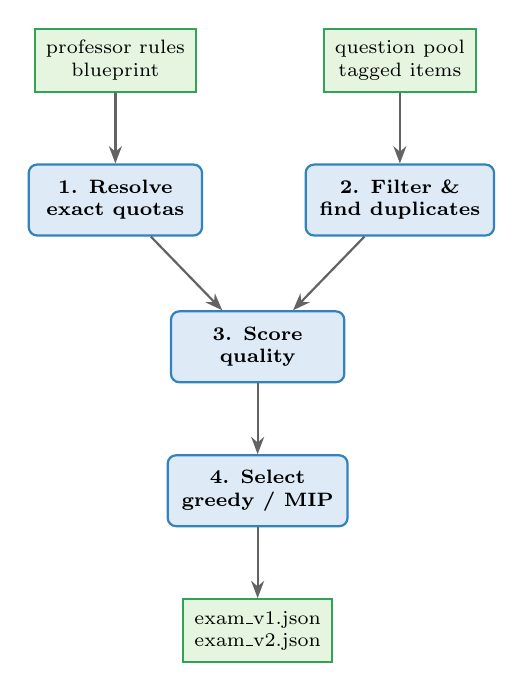
\begin{tikzpicture}[node distance=7mm and 10mm]
        \node[data] (rules) {professor rules\\blueprint};
        \node[data, right=16mm of rules] (pool) {question pool\\tagged items};
        \node[stage, below=9mm of rules] (resolve) {1. Resolve\\exact quotas};
        \node[stage, below=9mm of pool] (filter) {2. Filter \&\\find duplicates};
        \node[stage, below=14mm of $(resolve)!0.5!(filter)$] (score) {3. Score\\quality};
        \node[stage, below=9mm of score] (select) {4. Select\\greedy / MIP};
        \node[data, below=9mm of select] (out) {exam\_v1.json\\exam\_v2.json};
        \draw[arr] (rules) -- (resolve);
        \draw[arr] (pool) -- (filter);
        \draw[arr] (resolve) -- (score);
        \draw[arr] (filter) -- (score);
        \draw[arr] (score) -- (select);
        \draw[arr] (select) -- (out);
      \end{tikzpicture}}
    \end{column}
    \begin{column}{0.54\textwidth}
      \footnotesize
      \begin{enumerate}
        \item \textbf{Resolve} the blueprint into a normalised demand vector.
        \item \textbf{Filter} out disallowed types; detect near-duplicate pairs.
        \item \textbf{Score} each candidate's quality (a selection preference).
        \item \textbf{Select} complete versions — greedy or MIP.
      \end{enumerate}
    \end{column}
  \end{columns}
\end{frame}

% =====================================================================
\begin{frame}{Near-duplicate detection}
  Variants that differ by a phrase (\emph{``…(variant 1)''} vs
  \emph{``…(variant 2)''}) test the same content — they should not co-occur.

  \vspace{1mm}
  \textbf{Default backend — token-Jaccard} (dependency-free):
  \[
    \mathrm{sim}(q_1,q_2)=\frac{|T_1 \cap T_2|}{|T_1 \cup T_2|}\in[0,1]
  \]
  $T_i$ = lowercase word tokens from stem + answer + options.

  \begin{block}{Example}
    ``Define the term uninformed search'' vs the same + ``variant'':
    5 shared / 6 total $=5/6\approx0.833$. At threshold \textbf{0.85} this pair
    is \emph{not} blocked; $\geq 0.85$ adds it to the duplicate set $D$.
  \end{block}

  \footnotesize\textbf{Optional backend:} sentence-transformers embedding cosine
  — catches paraphrases that share little surface vocabulary.
\end{frame}

% =====================================================================
\begin{frame}{Scoring question quality}
  A lightweight \emph{preference} weight (not a correctness score), used only to
  break ties among feasible selections:
  \[
    w_i = 1.0 + b_{\text{expl}} + b_{\text{options}} + b_{\text{bloom}} + b_{\text{difficulty}}
  \]
  \begin{center}\footnotesize
  \begin{tabular}{@{}ll@{}}
    \toprule
    \textbf{Component} & \textbf{Rationale} \\
    \midrule
    Base $1.0$ & every valid question has minimal value \\
    Explanation bonus & longer explanations $\to$ auditability / feedback \\
    Options bonus & MCQ with exactly four options \\
    Bloom bonus & \code{analyze}/\code{evaluate}/\code{create} (higher order) \\
    Difficulty bonus & small bonus for hard items \\
    \bottomrule
  \end{tabular}
  \end{center}
  \vspace{1mm}
  \footnotesize\emph{e.g.} hard MCQ, Bloom \code{evaluate}, 4 options, long
  explanation: $1.0+0.30+0.20+0.20+0.10=\mathbf{1.80}$.
\end{frame}

% =====================================================================
\begin{frame}[fragile]{Step 4a — the greedy selector (baseline)}
  Builds one version, one chapter at a time; reproducible shuffle; difficulty-aware
  first pass, then fill; blocks near-duplicates after each pick.
\begin{lstlisting}
For each version:
  For each required chapter:
    collect candidates; drop used / near-duplicate-blocked; shuffle (seeded)
    pass 1: choose candidates that still help the difficulty quota
    pass 2: fill remaining chapter slots with any candidate
    mark chosen as used; block their near-duplicates
\end{lstlisting}
  \begin{columns}[T]
    \begin{column}{0.5\textwidth}
      \footnotesize\textbf{Strengths}
      \begin{itemize}
        \item Very fast, easy to inspect
        \item Honours exact chapter counts
      \end{itemize}
    \end{column}
    \begin{column}{0.5\textwidth}
      \footnotesize\textbf{Limitations}
      \begin{itemize}
        \item No global optimality
        \item Later versions get leftovers; difficulty only best-effort
      \end{itemize}
    \end{column}
  \end{columns}
\end{frame}

% =====================================================================
\begin{frame}{Step 4b — the MIP selector (default, exact)}
  Models the \textbf{whole} assembly at once — all questions, versions, quotas,
  exclusions, weights — as one 0--1 (Binary) Integer Program.

  \vspace{2mm}
  \textbf{Decision variables}
  \[
    x_{iv}\in\{0,1\}\quad\forall i\in\{0,\dots,n-1\},\;\forall v\in V
  \]
  ($x_{iv}=1$ iff question $i$ is placed in version $v$).

  \textbf{Objective — maximise total selected quality}
  \[
    \max\; Z = \sum_{v\in V}\sum_{i=0}^{n-1} w_i\,x_{iv}
  \]
  \footnotesize With 180 questions $\times$ 2 versions: 360 binary switches; the
  solver turns exactly the right ones on.
\end{frame}

% =====================================================================
\begin{frame}{MIP — the constraints}
  \begin{align*}
    \text{exact chapter counts:}\quad & \sum_{i\in Q_c} x_{iv}=n_c
      && \forall c\in C,\;\forall v\in V \\[1mm]
    \text{exact difficulty counts:}\quad & \sum_{i\in Q_l} x_{iv}=m_l
      && \forall l\in L,\;\forall v\in V \\[1mm]
    \text{disjoint versions:}\quad & \sum_{v\in V} x_{iv}\le 1
      && \forall i \\[1mm]
    \text{no near-duplicate pair:}\quad & \sum_{v\in V}x_{iv}+\sum_{v\in V}x_{jv}\le 1
      && \forall (i,j)\in D
  \end{align*}
  \vspace{1mm}
  \footnotesize Solved with \textbf{PuLP + CBC} via branch-and-bound: an LP
  relaxation gives upper bounds, fractional variables are branched to $0/1$, and
  dominated branches are pruned — avoiding enumeration of all $2^{n|V|}$
  settings.
\end{frame}

% =====================================================================
\begin{frame}{When the exact model is infeasible}
  Sometimes the pool cannot satisfy every constraint at once (e.g. too few hard
  questions remain). A \textbf{two-phase solve} handles it:

  \vspace{2mm}
  \begin{enumerate}
    \item Try the full model (chapter + difficulty + disjoint + duplicate).
    \item If infeasible, \textbf{drop the difficulty equalities} and re-solve —
          keeping chapter counts, version disjointness, and duplicate exclusions.
  \end{enumerate}

  \vspace{2mm}
  \begin{block}{Deliberate asymmetry}
    Chapter coverage is the \textbf{core content requirement} and is never
    silently violated. Difficulty balance is the \textbf{safer constraint to
    relax} — the run records \code{difficulty\_relaxed} in its diagnostics.
  \end{block}
\end{frame}

% =====================================================================
\begin{frame}{Greedy vs. MIP at a glance}
  \begin{center}\footnotesize
  \begin{tabular}{@{}p{3.0cm}p{3.6cm}p{4.0cm}@{}}
    \toprule
    \textbf{Feature} & \textbf{Greedy} & \textbf{MIP (default)} \\
    \midrule
    Decision style & incremental, per version/chapter & whole problem in one model \\
    Chapter counts & exact & exact \\
    Difficulty counts & best effort & exact unless relaxed \\
    Overlap / duplicates & avoided by blocking & mathematically forbidden \\
    Quality & not globally optimised & objective maximises total quality \\
    Best for & fast drafts, large pools & final assembly, tight pools, audit \\
    \bottomrule
  \end{tabular}
  \end{center}
  \vspace{2mm}
  \begin{center}
  \textbf{\color{faublue}One interface, two selectors} — same constraints, different guarantees.
  \end{center}
\end{frame}

% =====================================================================
\begin{frame}{Deduplication \& validation}
  \begin{columns}[T]
    \begin{column}{0.5\textwidth}
      \begin{block}{Deduplication (two levels)}
        \footnotesize
        \begin{itemize}
          \item \textbf{Pool-level} (\code{--dedup}): drop the later member of
                each near-duplicate pair before assembly.
          \item \textbf{Selector-level}: forbid surviving pairs $D$ during
                version construction — a second line of defence.
        \end{itemize}
      \end{block}
    \end{column}
    \begin{column}{0.5\textwidth}
      \begin{block}{Validation (\code{--validate})}
        \footnotesize A structured report over four dimensions:
        \begin{enumerate}
          \item \textbf{Schema} validity (round-trips the model)
          \item \textbf{Blueprint} compliance (counts match \emph{exactly})
          \item \textbf{Grounding} coverage (\code{source\_ref} / overlap)
          \item \textbf{Duplicate} rate
        \end{enumerate}
        \vspace{1mm}
        Gate \code{passed} = no invalid items \emph{and} blueprint satisfied.
      \end{block}
    \end{column}
  \end{columns}
\end{frame}

% =====================================================================
\begin{frame}[fragile]{Command-line interface}
  One entry point: \pkg{\_\_main\_\_.py} — pool + blueprint/flags
  $\to$ one \code{Quiz} JSON per version (each embedding the resolved blueprint).
\begin{lstlisting}[language=bash]
# Pure command line: 20 questions, 10/6/4 across chapters,
# 40/40/20 difficulty, two disjoint versions, optimal (MIP):
python -m quizgen --pool questions.json \
    --total 20 --chapters 1:10,2:6,3:4 \
    --difficulty 0.4,0.4,0.2 --versions 2 --selector mip

# Blueprint file + dedup + per-version validation report:
python -m quizgen --pool questions.json --blueprint blueprint.yaml \
    --dedup --validate --out-dir out
\end{lstlisting}
  \footnotesize Flags \textbf{override} the YAML file. Exits non-zero if any
  version is non-compliant, so it composes in scripts and CI.
\end{frame}

% =====================================================================
\begin{frame}{Provenance of techniques}
  \begin{center}\footnotesize
  \begin{tabular}{@{}p{3.4cm}p{3.5cm}p{4.2cm}@{}}
    \toprule
    \textbf{In code} & \textbf{Technique} & \textbf{Source lineage} \\
    \midrule
    \pkg{assemble.py} MIP & ATA as a 0--1 MIP & van der Linden, \emph{Linear Models for Optimal Test Design} (2005) \\
    quality objective & objective-weighted selection & van der Linden (2005); here a quality proxy \\
    \pkg{blueprint.py} & table of specifications & classical assessment design \\
    \code{bloom\_level} & revised Bloom taxonomy & Anderson \& Krathwohl (2001); Bloom (1956) \\
    embedding dedup & semantic near-dup detection & Reimers \& Gurevych (2019), S-BERT \\
    \midrule
    \multicolumn{3}{@{}l}{\emph{Project engineering:} largest-remainder apportionment,}\\
    \multicolumn{3}{@{}l}{greedy baseline, Jaccard fallback, YAML+flag override precedence.}\\
    \bottomrule
  \end{tabular}
  \end{center}
\end{frame}

% =====================================================================
\begin{frame}{Summary}
  \begin{itemize}
    \item \textbf{quizgen implements the \emph{selection} half} of automated exam
          construction as an \textbf{exact optimisation problem}.
    \item Given a tagged question bank + a blueprint, it assembles
          \textbf{blueprint-compliant, mutually disjoint} versions via a
          \textbf{0--1 MIP}, with a greedy baseline behind the same interface.
    \item An optional \textbf{dedup} pass and a layered \textbf{validation}
          report (schema, blueprint, grounding, duplicates) verify the result.
    \item \alert{No LLM, no document processing} — fully offline; constraints via
          a blueprint file and/or CLI flags.
  \end{itemize}

  \vfill
  \begin{center}
    {\color{faublue}\rule{0.5\textwidth}{1pt}}\\[2mm]
    {\large\bfseries\color{faublue}Thank you — questions?}\\[1mm]
    {\footnotesize Jiniku Hayashi \,·\, KWARC \,·\, FAU Erlangen-Nürnberg}
  \end{center}
\end{frame}

\end{document}
